\section{Dataset Generation (Extended)}\label{app:datGeneration}

Due to structural differences between graphs generated by the two generation procedures for experiment 1, the resulting graphs naturally exhibit markedly different average degrees.
In particular, graphs containing a $k$-clique tend to have higher average degree than $(k\!-\!1)$-colorable graphs. %This can be shown analytically.

As a consequence, the two classes can often be separated by simple statistics such as average degree, making this setting comparatively easy for graph neural networks. %(This is discussed in more detail in section \ref{subsec:ResultsandDiscussion}). 
This observation immediately motivates a more constrained experimental setting.

The average degree of clique implanted graphs is given by,

\begin{equation}
\label{eq:s-edgeprob}
    \begin{split}
        d_{avg} = \frac{s(s-1) + 2sq(n-s) + q (n -s) (n-s-1) }{n}
    \end{split}
\end{equation}

while the average degree of $n$-node color class implanted graphs is given by, 

\begin{equation}
\label{eq:r-edgeprob}
    \begin{split}
        d_{avg} = p(n-1)\frac{(r-1)}{r}.
    \end{split}
\end{equation}

Combining equations \ref{eq:r-edgeprob} and \ref{eq:s-edgeprob} gives a probability $p$ generating clique implanted graphs and color class implanted graphs with matching average (expected) degrees. 
As a result, the empirical degree distributions of the two classes become nearly indistinguishable, while the underlying clique versus coloring structure is preserved (see figure \ref{fig:same-dist}). 

\begin{figure}[htbp]
    \centering
    \begin{subfigure}[t]{0.48\linewidth}
        \centering
        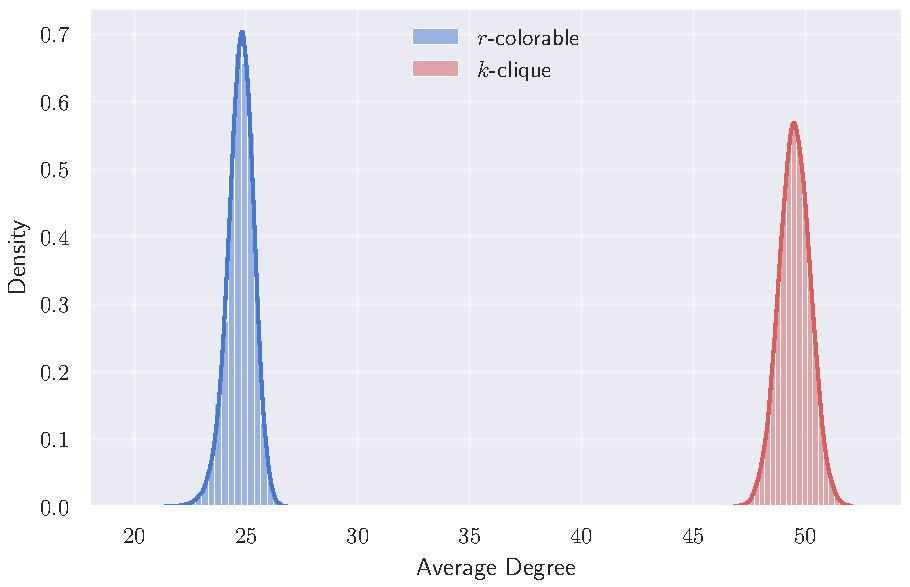
\includegraphics[width=\linewidth]{sketches/plots/same-edgeprob.pdf}
        \caption{Histogram with KDE of average degrees for 2-colorable and 3-clique graphs with $N=100$ and $p=0.5$.}
        \label{fig:avg-degrees}
    \end{subfigure}
    \hfill
    \begin{subfigure}[t]{0.48\linewidth}
        \centering
        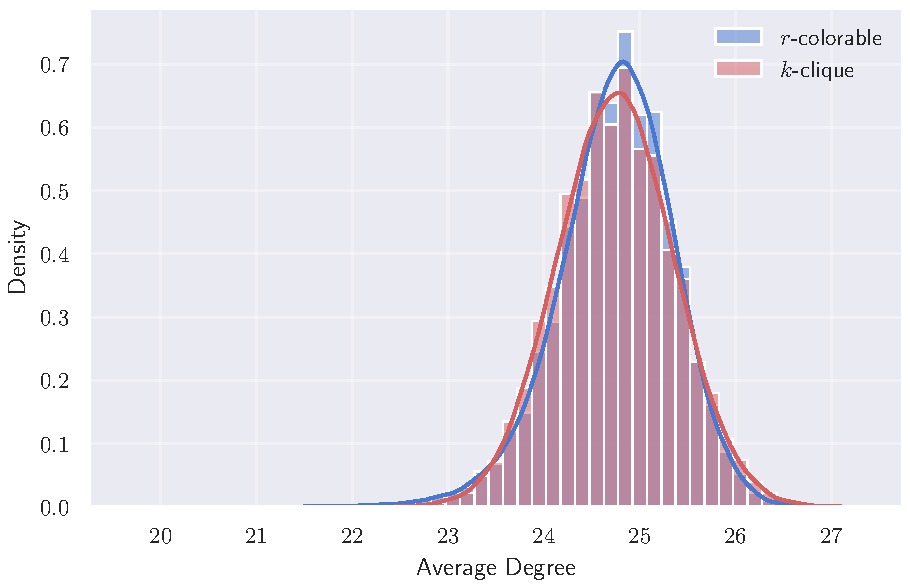
\includegraphics[width=\linewidth]{sketches/plots/same-dist.pdf}
        \caption{Histogram with KDE of average degrees for 2-colorable and 3-clique graphs with $N=100$ and adjusted edge probability.}
        \label{fig:same-dist}
    \end{subfigure}
    \caption{Comparison of average-degree distributions under matched-degree sampling (right) and fixed $p=0.5$ (left).}
\end{figure}


% \begin{figure}[htbp]
%     \centering
%     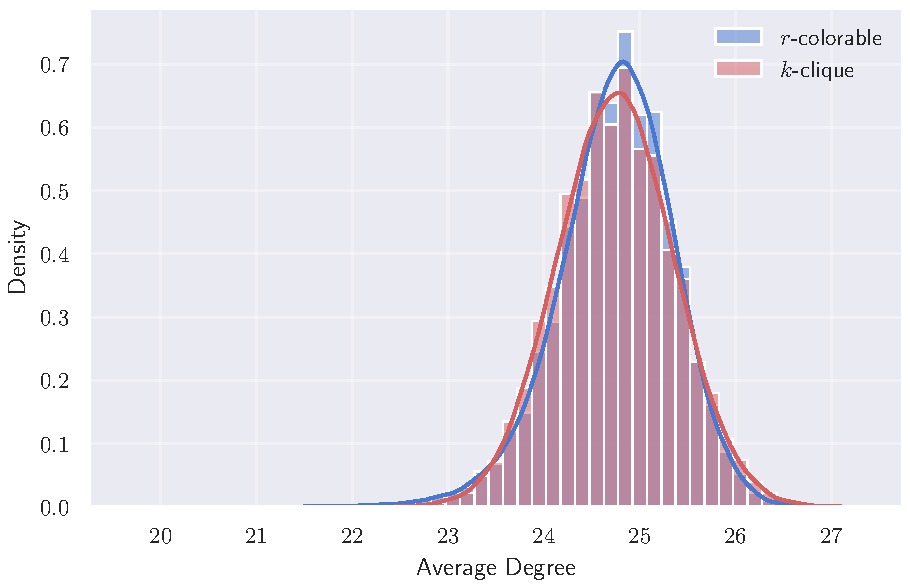
\includegraphics[width=0.9\linewidth]{sketches/plots/same-dist.pdf}
%     \caption{Histogram with KDE of average degrees for 2-colorable and 3-clique graphs with $N = 100$ and edge probability adjusted to give the same average degree.}
%     \label{fig:same-dist}
% \end{figure}

% \begin{figure}[h]
%     \centering
%     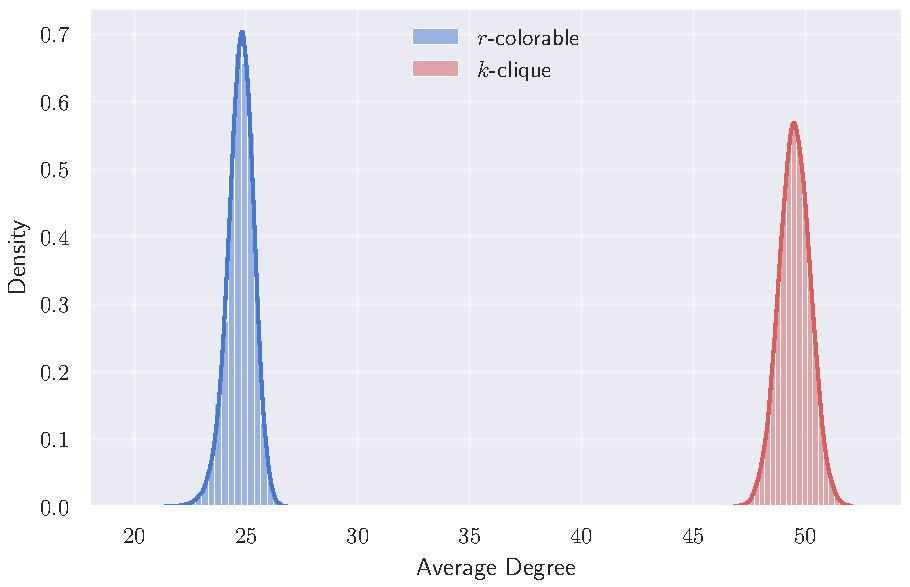
\includegraphics[width=0.9\linewidth]{sketches/plots/same-edgeprob.pdf}
%     \caption{Histogram with KDE of average degrees for 2-colorable and 3-clique graphs with $N = 100$ and $p = 0.5$}
%     \label{fig:avg-degrees}
% \end{figure}
